\documentclass{article}
\usepackage{graphicx}
\usepackage[margin=1.5cm]{geometry}
\usepackage{amsmath}

\begin{document}
\twocolumn

\title{Tuesday Warm Up, Unit 1: Filter Design}
\author{Prof. Jordan C. Hanson}
\maketitle

\section{Memory Bank}
\small
\begin{itemize}
\item \textbf{Convolution}: this is an operation that characterizes the response $h[n]$ of a linear system.
\begin{equation}
y[i] = h[n] * x[n] = \sum_{j=0}^{M-1}h[j]x[i-j] \label{eq:conv}
\end{equation}
In words, the output at sample $i$ is equal to the produce of the system response $h$ and the input signal $x$, summed over the proceeding $M$ samples (from $j=0$ to $j=M-1$).
\item \textbf{Discrete Delta Function}, $\delta[n]$: A standard impulse response that contains one non-zero sample.  It has the following property:
\begin{equation}
x[n] = \delta[n] * x[n] \label{eq:conv2}
\end{equation}
\item The \textbf{filter kernel} is the impulse response of a digital filter.  Convolve this with the signal to obtain the output.
\item \textbf{IIR} - infinite impulse response.  A filter response can decay exponentially, never reaching zero.
\item \textbf{FIR} - finite impulse response.  A digital filter can be implemented via a kernel with a finite set of coefficients.
\item \textbf{Decibels} - $dB = 10\log_{10}(P_2/P_1) = 20\log_{10}(A_2/A_1)$ ... A decibel unit of attenuation or amplification is a logarithmic unit of amplitude ratios $A_i$ or power ratios $P_i$.
\end{itemize}

\section{Basic Filter Concepts}

\begin{enumerate}
\item (a) Suppose a filter lowers a signal amplitude from 5 V to 5 mV at 15 kHz.  What is this attenuation in dB? (b) Suppose a filter lowers signal amplitude by 40 dB in the stop band.  If the input signal amplitude is 12 V, what is the output amplitude? (c) We need to amplify a signal from 10 $\mu$W to 100 mW.  What power amplification is required, in dB? (d) A \textbf{dBm} is a decibel unit in which the power in the denominator is set to 1 mW exactly.  RF thermal noise in amplified RF antennas is usually observed to be -174 dBm.  What is this power in regular units? \\ \vspace{2.5cm}
\item Consider Fig. \ref{fig:1}, which contains the step response of a filter.  (a) Assume the sampling frequency is 2 MHz.  What is the time duration from sample 0 to sample 64? (b) Estimate the \textit{rise-time} of the step response. \\ \vspace{1cm}
\end{enumerate}

\section{Mathematics of Filter Response}

\begin{enumerate}
\item Let $y[n]$ be the output of a filter.  The output $y[n]$ is equal to $h[n]$ when the input is $\delta[n]$.  (a) Prove that the \textit{step response} is the running sum of $h[n]$. (b) Prove that the impulse is the discrete derivative (first-difference) of the step response. \\ \vspace{2.5cm}
\item Using \verb+octave+, create a low-pass filter kernel with 16 samples, called \verb+k+. To ensure it is low-pass, make it a smoothly rising and falling function.  Compute the following: (a) the impulse response of \verb+k+, and (b) the step response of \verb+k+.
\item \textbf{Spectral inversion} of a filter kernel changes its behavior from low-pass to high-pass.  Using your kernel from the previous exercise, create a high-pass kernel by subtracting it from an impulse at sample zero. Compute the following: (a) the new impulse response, and (b) the new step response.  \textbf{Graph the responses from this and the previous exercise below.}
\end{enumerate}

\begin{figure}
\centering
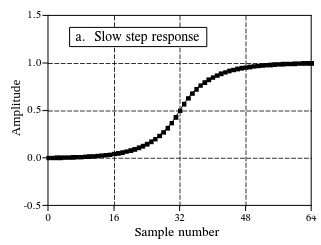
\includegraphics[width=0.35\textwidth]{step.png}
\caption{\label{fig:1} Example of a filter kernel with a slow rise-time.}
\end{figure}

\end{document}
